% CVPR 2022 Paper Template
% based on the CVPR template provided by Ming-Ming Cheng (https://github.com/MCG-NKU/CVPR_Template)
% modified and extended by Stefan Roth (stefan.roth@NOSPAMtu-darmstadt.de)

\documentclass[10pt,twocolumn,letterpaper]{article}

%%%%%%%%% PAPER TYPE  - PLEASE UPDATE FOR FINAL VERSION %%%%%%%%%
%\usepackage[review]{cvpr}      % To produce the REVIEW version
%\usepackage{cvpr}              % To produce the CAMERA-READY version
\usepackage[pagenumbers]{cvpr} % To force page numbers, e.g. for an arXiv version

% Include other packages here, before hyperref.
\usepackage{graphicx}
\usepackage{amsmath}
\usepackage{amssymb}
\usepackage{booktabs}
\usepackage{float}
\usepackage{arydshln}


% It is strongly recommended to use hyperref, especially for the review version.
% hyperref with option pagebackref eases the reviewers' job.
% Please disable hyperref *only* if you encounter grave issues, e.g. with the
% file validation for the camera-ready version.
%
% If you comment hyperref and then uncomment it, you should delete
% ReviewTempalte.aux before re-running LaTeX.
% (Or just hit 'q' on the first LaTeX run, let it finish, and you
%  should be clear).
\usepackage[pagebackref,breaklinks,colorlinks]{hyperref}


% Support for easy cross-referencing
\usepackage[capitalize]{cleveref}
\crefname{section}{Sec.}{Secs.}
\Crefname{section}{Section}{Sections}
\Crefname{table}{Table}{Tables}
\crefname{table}{Tab.}{Tabs.}

\raggedbottom
\begin{document}

%%%%%%%%% TITLE - PLEASE UPDATE %%%%%%%%%
\title{DLP Lab1: Backpropagation}

\author{Yi-Hsiang Ho, 111550106
% For a paper whose authors are all at the same institution,
% omit the following lines up until the closing ``}''.
% Additional authors and addresses can be added with ``\and'',
% just like the second author.
% To save space, use either the email address or home page, not both
% \and
% Second Author\\
% Institution2\\
% First line of institution2 address\\
% {\tt\small secondauthor@i2.org}
}
\maketitle

%%%%%%%%% BODY TEXT %%%%%%%%%

% ------------------------- Introduction -------------------------

\section{Introduction}
\label{sec:intro}

In this lab, we need to build a Multi-Layer Perceptron (MLP) from scratch using only
NumPy, without modern deep learning frameworks. The primary objective is to
acquire hands-on understanding of the backpropagation algorithm by explicitly
deriving and implementing the forward and backward passes.

The neural network is trained and evaluated on two binary classification tasks:
a linearly separable dataset and the non-linearly separable XOR dataset. By
constructing a complete training pipeline, including forward propagation, loss
computation, and gradient descent, we may demonstrate how multi-layer
architectures solve non-linear problems and understand the inner workings
of neural network training.


% -------------------- Implementation Details --------------------

\section{Implementation Details}
\label{sec:impl}

\subsection{Sigmoid Function}
\label{subsec:sigmoid}

The sigmoid function squashes inputs into $(0, 1)$ for binary 
classification probabilities. Its forward pass is:
\begin{equation}
  \sigma(x) = \frac{1}{1 + e^{-x}}
\end{equation}

By the quotient rule, the derivative for the backward pass is:
\begin{equation}
  \frac{\partial \sigma(x)}{\partial x} = \sigma(x) \cdot (1 - \sigma(x))
\end{equation}

The implementation is as follows:

\begin{figure}[H]
  \centering
  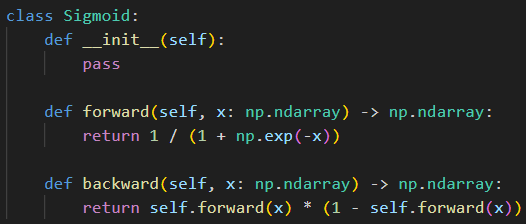
\includegraphics[width=\linewidth]{assets/impl-sigmoid.png}
  \caption{\textbf{The implementation of sigmoid funciton class}}
  \label{fig:impl-sigmoid}
\end{figure}


\subsection{Neural network architecture}

The architecture of the neural network can be formulated as:
\begin{equation}
  \begin{aligned}
    z_1 &= \mathbf{W}_1 \mathbf{x} + \mathbf{b}_1, \\
    \mathbf{h}_1 &= \sigma(z_1), \\
    z_2 &= \mathbf{W}_2 \mathbf{h}_1 + \mathbf{b}_2, \\
    \mathbf{h}_2 &= \sigma(z_2), \\
    z_3 &= \mathbf{W}_3 \mathbf{h}_2 + \mathbf{b}_3, \\
    y &= \sigma(z_3)
  \end{aligned}
\end{equation}
where $\mathbf{W}_1$, $\mathbf{W}_2$, and $\mathbf{W}_3$ are the weight
matrices, $\mathbf{b}_1$, $\mathbf{b}_2$, and $\mathbf{b}_3$ are the bias
vectors, and $\sigma$ is the sigmoid function.

Each layer is wrapped into a class. The implementation of linear layer
is in \cref{fig:impl-linear}. The implementation of the
network is in \cref{fig:impl-net}.

\begin{figure}[H]
  \centering
  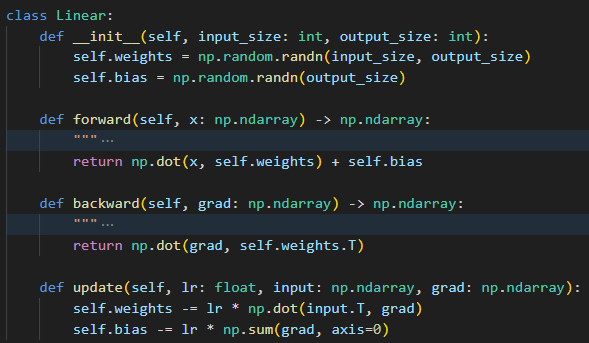
\includegraphics[width=\linewidth]{assets/impl-linear.png}
  \caption{\textbf{The implementation of linear layer class}}
  \label{fig:impl-linear}
\end{figure}

\begin{figure}[H]
  \centering
  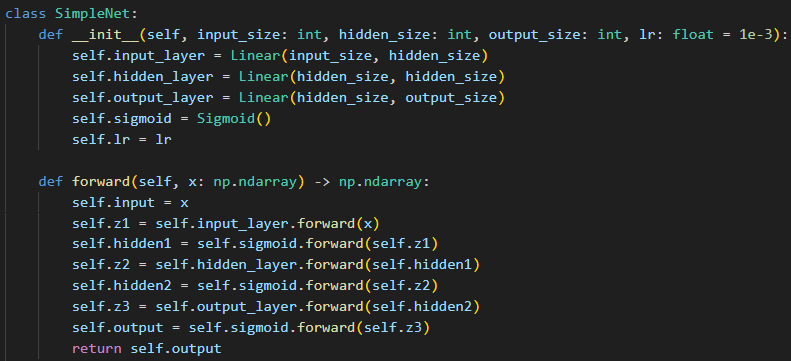
\includegraphics[width=\linewidth]{assets/impl-net.png}
  \caption{\textbf{The implementation of neural network architecture}}
  \label{fig:impl-net}
\end{figure}

\subsection{Backpropagation}

Given the loss gradient with respect to the network output
$\frac{\partial L}{\partial y}$, backpropagation computes the gradient
for each layer using the chain rule. The gradients with respect to the
pre-activations $z_3, z_2$, and $z_1$ are computed as follows:
\begin{equation}
  \begin{aligned}
    \frac{\partial L}{\partial z_3} &= \frac{\partial L}{\partial y} \odot \sigma'(z_3), \\
    \frac{\partial L}{\partial z_2} &= \left( \frac{\partial L}{\partial z_3} \mathbf{W}_3^T \right) \odot \sigma'(z_2), \\
    \frac{\partial L}{\partial z_1} &= \left( \frac{\partial L}{\partial z_2} \mathbf{W}_2^T \right) \odot \sigma'(z_1)
  \end{aligned}
\end{equation}
where $\odot$ denotes element-wise multiplication.

With these gradients, the network parameters for each layer
$l \in \{1, 2, 3\}$ are updated via gradient descent:
\begin{equation}
  \begin{aligned}
    \mathbf{W}_l &\leftarrow \mathbf{W}_l - \eta \left( \mathbf{h}_{l-1}^T \frac{\partial L}{\partial z_l} \right), \\
    \mathbf{b}_l &\leftarrow \mathbf{b}_l - \eta \sum \frac{\partial L}{\partial z_l}
  \end{aligned}
\end{equation}
where $\eta$ is the learning rate, $\mathbf{h}_0 = \mathbf{x}$, and
the sum for the bias gradient is taken over the batch dimension.

The implementation of backpropagation and weight update is combined in
the implementation of each layer, as shown in
\cref{fig:impl-backprop} and \cref{fig:impl-backprop-nn}.

\begin{figure}[H]
  \centering
  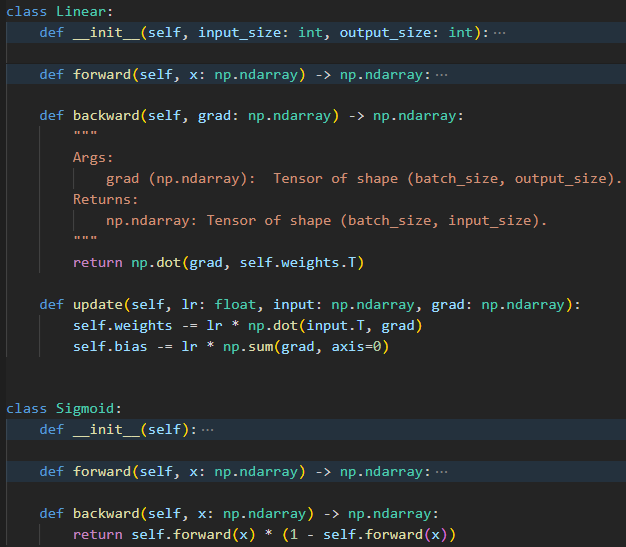
\includegraphics[width=\linewidth]{assets/impl-backprop.png}
  \caption{\textbf{The implementation of backpropagation}}
  \label{fig:impl-backprop}
\end{figure}

\begin{figure}[H]
  \centering
  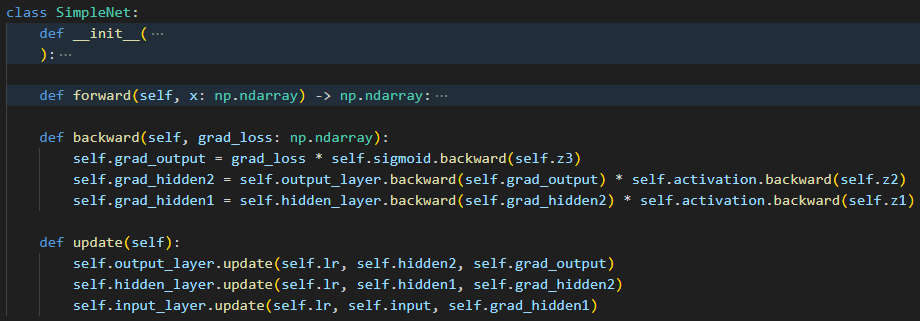
\includegraphics[width=\linewidth]{assets/impl-backprop-nn.png}
  \caption{\textbf{The implementation of backpropagation in neural network}}
  \label{fig:impl-backprop-nn}
\end{figure}

\subsection{Others}

In my implementation, the network supports batch processing, which means
that the network can process multiple samples at once. This is achieved by
using numpy's matrix operations. In default, the batch size is the total
number of samples, which is $1000$.

During inference, the network is used to predict the class of each sample.
if the output value is greater than $0.5$, the class is $1$, otherwise the
class is $0$.

% --------------------- Experimental Results ---------------------

\section{Experimental Results}

\subsection{Settings}
\label{subsec:settings}

\begin{table}[H]
  \centering
  \begin{tabular}{ll}
    \hline
    Setting & Value \\
    \hline
    Learning rate & $5 \times 10^{-3}$ \\
    Hidden layer size & $16$ \\
    Epochs & $10000$ \\
    Number of training data (in linear dataset) & $1000$ \\
    Number of testing data (in linear dataset) & $100$ \\
    \hline
  \end{tabular}
\end{table}

\subsection{Comparison figure}

\begin{figure}[H]
  \centering
  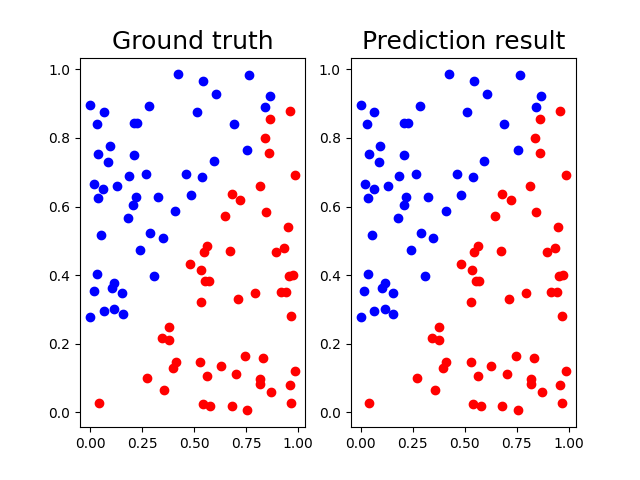
\includegraphics[width=0.9\linewidth]{assets/result-linear.png}
  \caption{\textbf{Comparison figure of linear dataset}}
  \label{fig:result_linear}
\end{figure}

\begin{figure}[H]
  \centering
  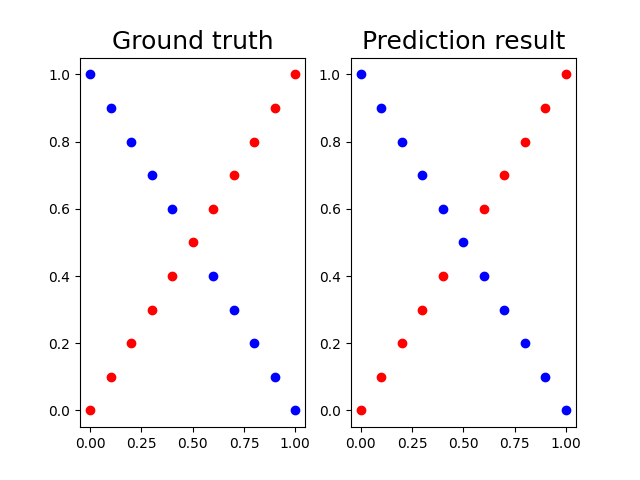
\includegraphics[width=0.9\linewidth]{assets/result-XOR.png}
  \caption{\textbf{Comparison figure of XOR dataset}}
  \label{fig:result_xor}
\end{figure}

\subsection{Accuracy}

\begin{figure}[H]
  \centering
  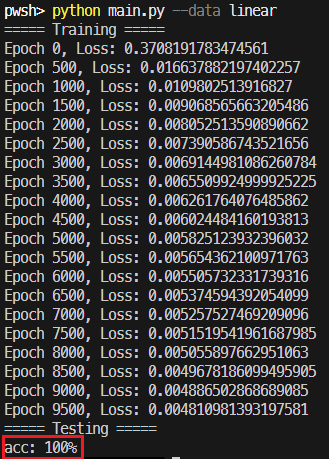
\includegraphics[width=0.9\linewidth]{assets/acc-linear.png}
  \caption{\textbf{Accuracy of linear dataset}}
  \label{fig:accuracy_linear}
\end{figure}

\begin{figure}[H]
  \centering
  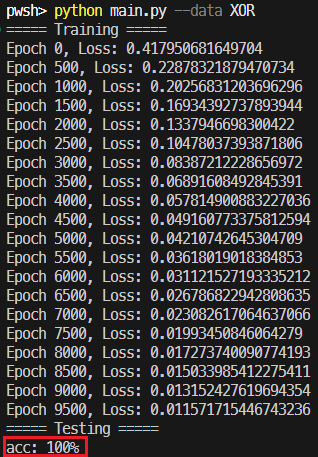
\includegraphics[width=0.9\linewidth]{assets/acc-XOR.png}
  \caption{\textbf{Accuracy of XOR dataset}}
  \label{fig:accuracy_xor}
\end{figure}

\subsection{Learning Curve}

\begin{figure}[H]
  \centering
  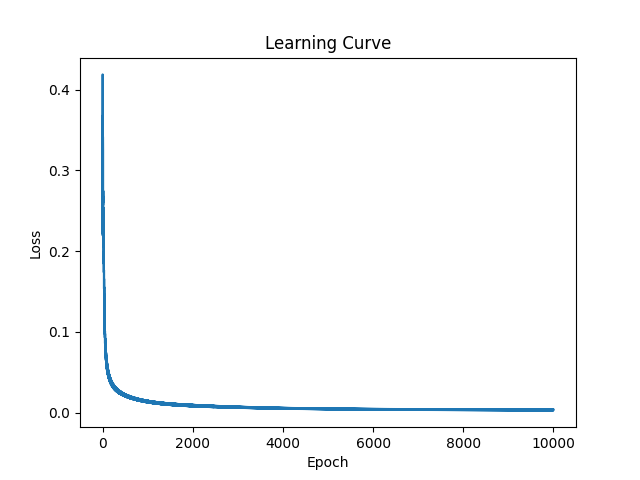
\includegraphics[width=0.9\linewidth]{assets/learning_curve-linear.png}
  \caption{\textbf{Learning curve of linear dataset}}
  \label{fig:learning_curve_linear}
\end{figure}

\begin{figure}[H]
  \centering
  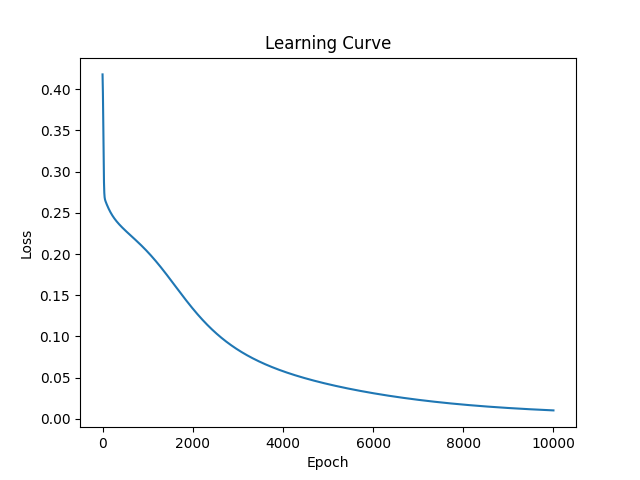
\includegraphics[width=0.9\linewidth]{assets/learning_curve-XOR.png}
  \caption{\textbf{Learning curve of XOR dataset}}
  \label{fig:learning_curve_xor}
\end{figure}

% -------------------------- Discussion --------------------------

\section{Discussion}

Note that the experiments below follow the settings in \cref{subsec:settings},
except for the target variable.

% ----- Different Learning Rates -----

\subsection{Different Learning Rates}

The learning rate (LR) determines the step size during gradient descent.
The results are shown in \cref{fig:learning_curve_exp_lr_XOR},
\cref{fig:result_exp_lr_XOR}, \cref{fig:learning_curve_exp_lr_linear},
and \cref{fig:result_exp_lr_linear}.
From the experiments with $\eta \in \{0.1, 0.01, 0.001, 0.0001\}$:
\begin{itemize}
    \item \textbf{High LR (0.1, 0.01):} The learning process is quite fast.
      They successfully converge on XOR dataset and gain $100\%$ accuracy.
      However, in linear dataset, $\eta=0.01$ still converges fast, but
      $\eta=0.1$ fails to converge, staying at $50\%$ accuracy. This
      occurs because the large learning rate, combined with a batch size of
      $1000$ samples, produces an massive weight update in the initial steps.
      This magnitude pushes the weights into the saturation region of
      the Sigmoid function, where the derivative
      $\sigma'(z) = \sigma(z)(1-\sigma(z))$ is nearly zero. Consequently, the
      gradients vanish, and the model's weights stop updating, leaving it stuck
      in a state of poor performance.

    \item \textbf{Low LR (0.001, 0.0001):} The learning process is much
      slower. Within 10,000 epochs, both two cases cannot converge on XOR
      dataset, and the accuracy is $71\%$ and $33\%$, respectively. On the
      other hand, in linear dataset, both two cases converge successfully,
      but in a slower speed.
\end{itemize}

\begin{figure}[H]
  \centering
  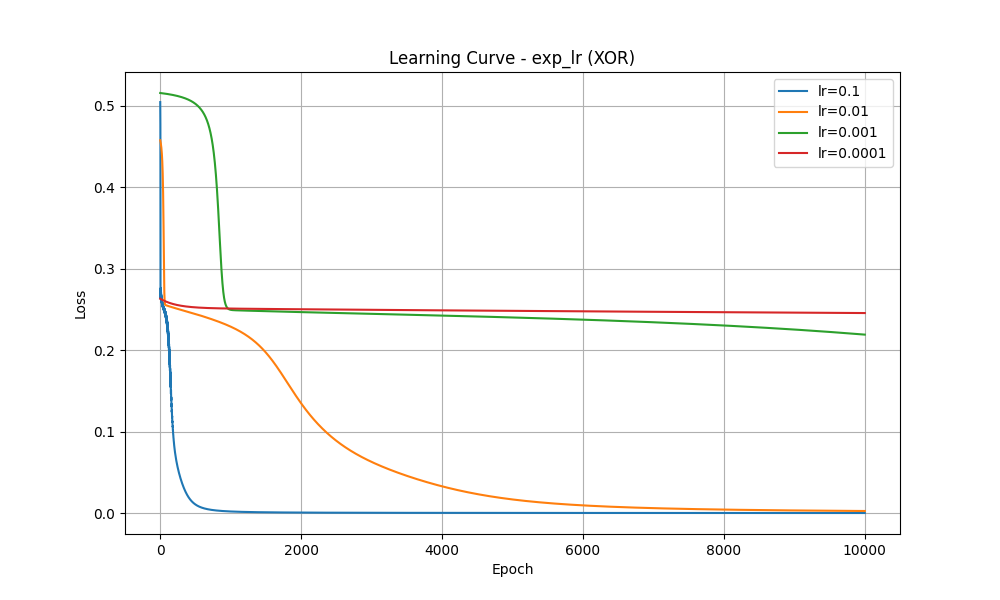
\includegraphics[width=\linewidth]{assets/learning_curve_exp_lr_XOR.png}
  \caption{\textbf{Learning curves for different learning rates on XOR dataset}}
  \label{fig:learning_curve_exp_lr_XOR}
\end{figure}

\begin{figure}[H]
  \centering
  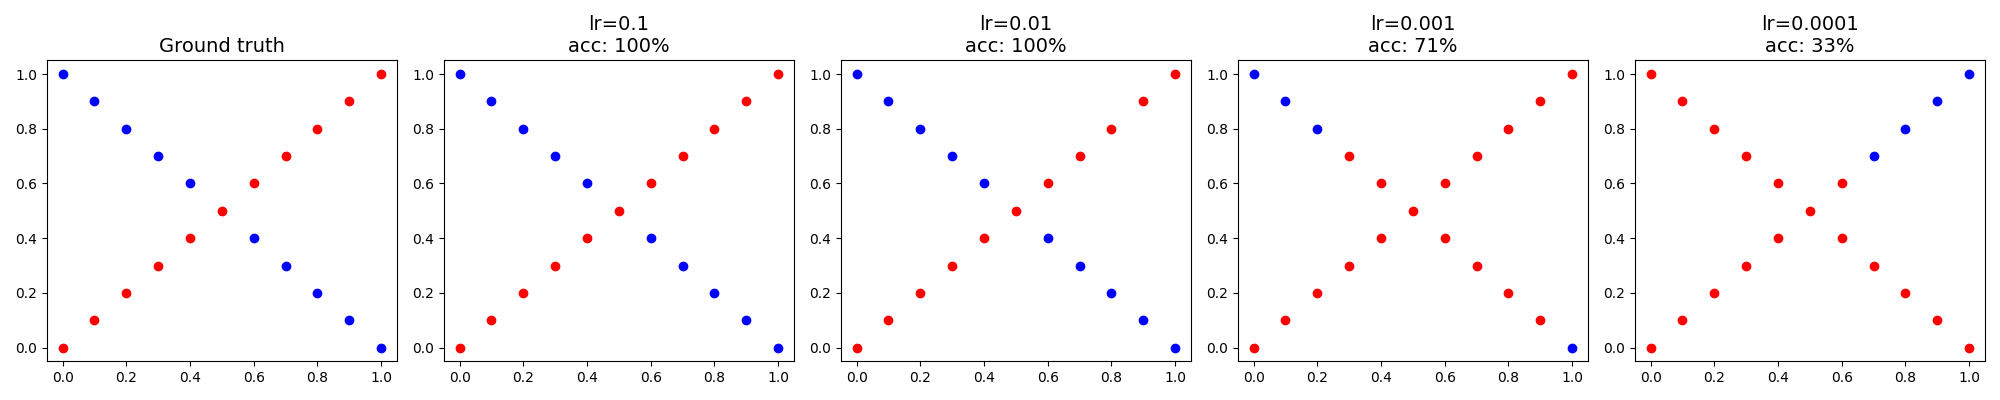
\includegraphics[width=\linewidth]{assets/result_exp_lr_XOR.png}
  \caption{\textbf{Prediction results for different learning rates on XOR dataset}}
  \label{fig:result_exp_lr_XOR}
\end{figure}

\begin{figure}[H]
  \centering
  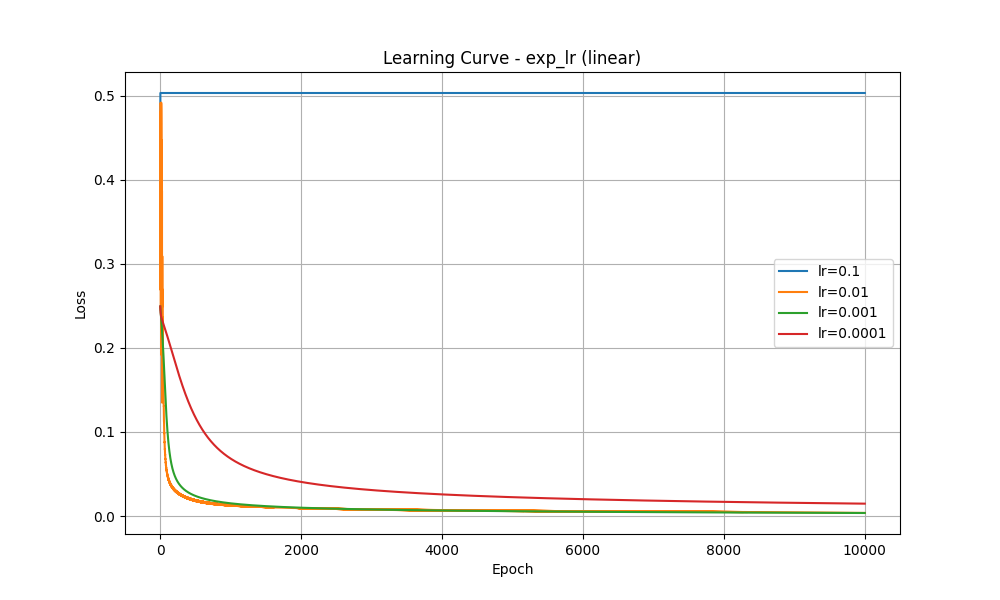
\includegraphics[width=\linewidth]{assets/learning_curve_exp_lr_linear.png}
  \caption{\textbf{Learning curves for different learning rates on linear dataset}}
  \label{fig:learning_curve_exp_lr_linear}
\end{figure}

\begin{figure}[H]
  \centering
  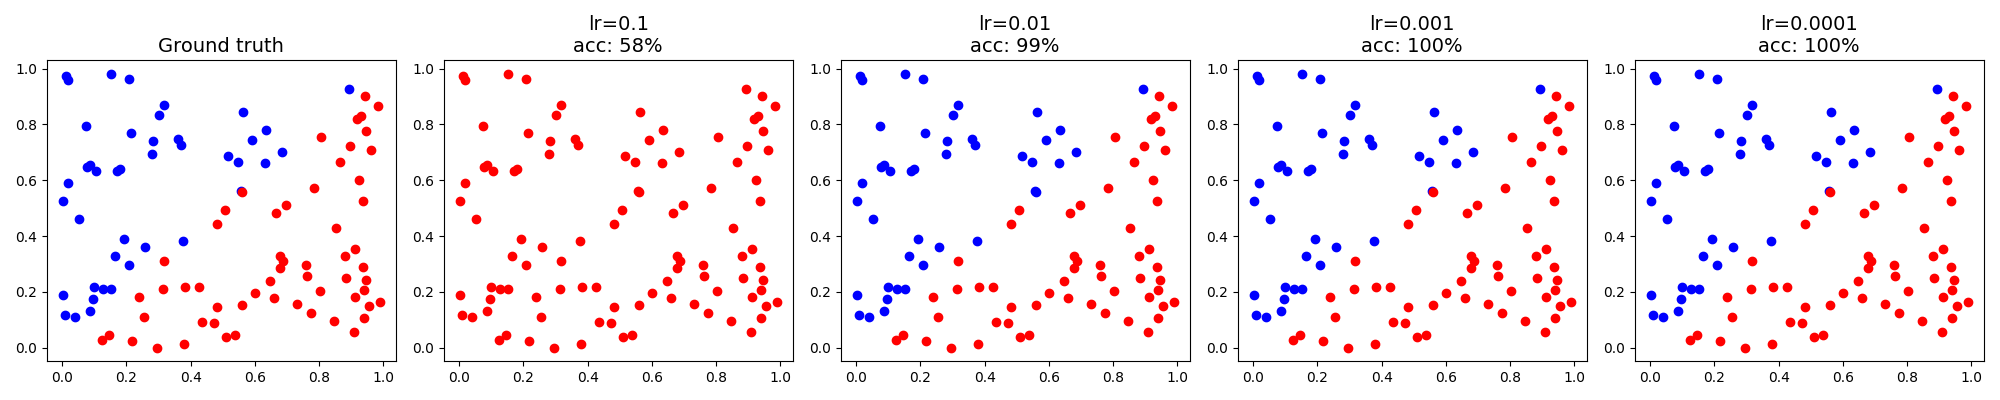
\includegraphics[width=\linewidth]{assets/result_exp_lr_linear.png}
  \caption{\textbf{Prediction results for different learning rates on linear dataset}}
  \label{fig:result_exp_lr_linear}
\end{figure}

% ----- Different Number of Hidden Units -----

\subsection{Different Number of Hidden Units}

The number of hidden units represents the model's capacity to learn complex patterns.
I tested $hs \in \{4, 16, 64, 256\}$, as shown in
\cref{fig:learning_curve_exp_hs_XOR}, \cref{fig:result_exp_hs_XOR},
\cref{fig:learning_curve_exp_hs_linear}, and \cref{fig:result_exp_hs_linear}:
\begin{itemize}
    \item \textbf{Small capacity ($hs=4$):} The model has limited
      representational power. While it still solves the linear and XOR
      problems, it converges slower than the larger models.
    \item \textbf{Large capacity ($hs=16, 64, 256$):} These models converge more rapidly
      in XOR dataset. However, the computational cost per epoch also increases significantly.
\end{itemize}

\begin{figure}[H]
  \centering
  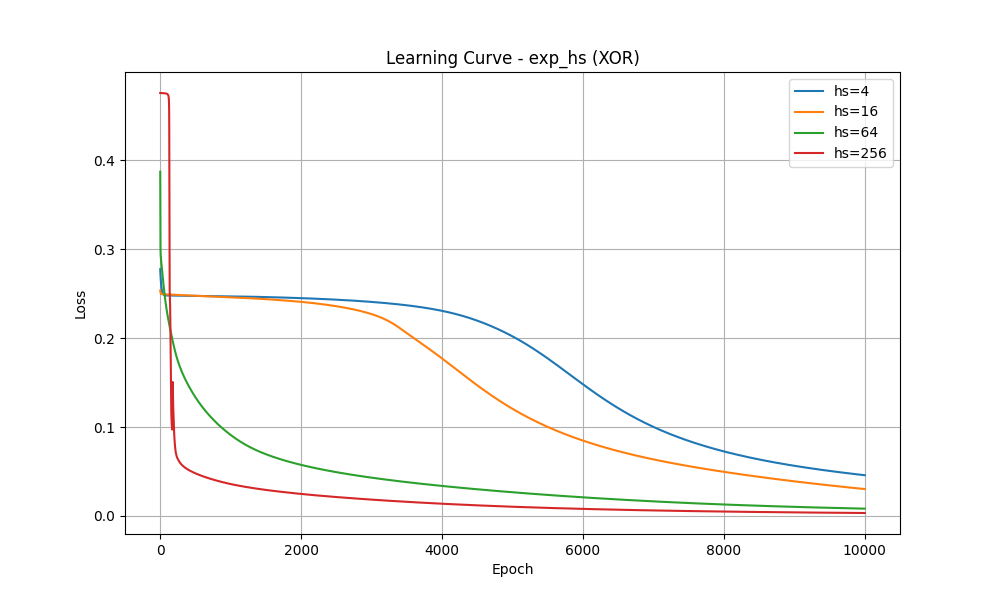
\includegraphics[width=\linewidth]{assets/learning_curve_exp_hs_XOR.png}
  \caption{\textbf{Learning curves for different number of hidden units on XOR dataset}}
  \label{fig:learning_curve_exp_hs_XOR}
\end{figure}

\begin{figure}[H]
  \centering
  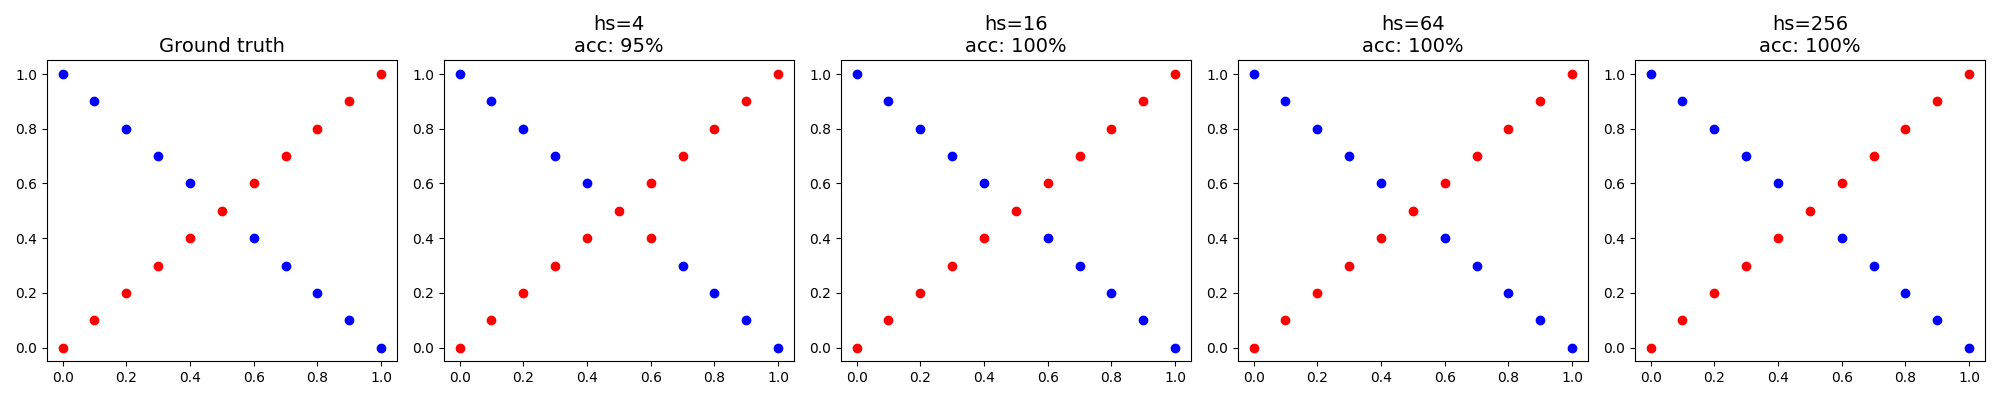
\includegraphics[width=\linewidth]{assets/result_exp_hs_XOR.png}
  \caption{\textbf{Prediction results for different number of hidden units on XOR dataset}}
  \label{fig:result_exp_hs_XOR}
\end{figure}

However, more hidden units mean more parameters to be learned, which significantly 
increases the model's complexity. In the linear dataset, we can see that the 
performance surprisingly drops at $hs=64$, failing to converge. This is a 
result of the unscaled random initialization ($\mathcal{N}(0, 1)$) 
combined with the Sigmoid activation. As the number of hidden units 
increases, the variance of the pre-activations $z = \mathbf{W}\mathbf{h} + \mathbf{b}$ 
also increases, pushing the hidden units into the saturation region where 
the gradient vanishes. 

Interestingly, at $hs=256$, the loss oscillates erraticly, but the model eventually
manages to converge to $100\%$ accuracy. This suggests that with a sufficiently
large number of parameters, the optimization landscape becomes more chaotic, and
these oscillations can occasionally ``kick'' the network out of saturated states,
allowing it to eventually find a path to convergence. In contrast, at $hs=64$,
the network remains trapped in a dead state from which it cannot recover within
the given 10,000 epochs.

\begin{figure}[H]
  \centering
  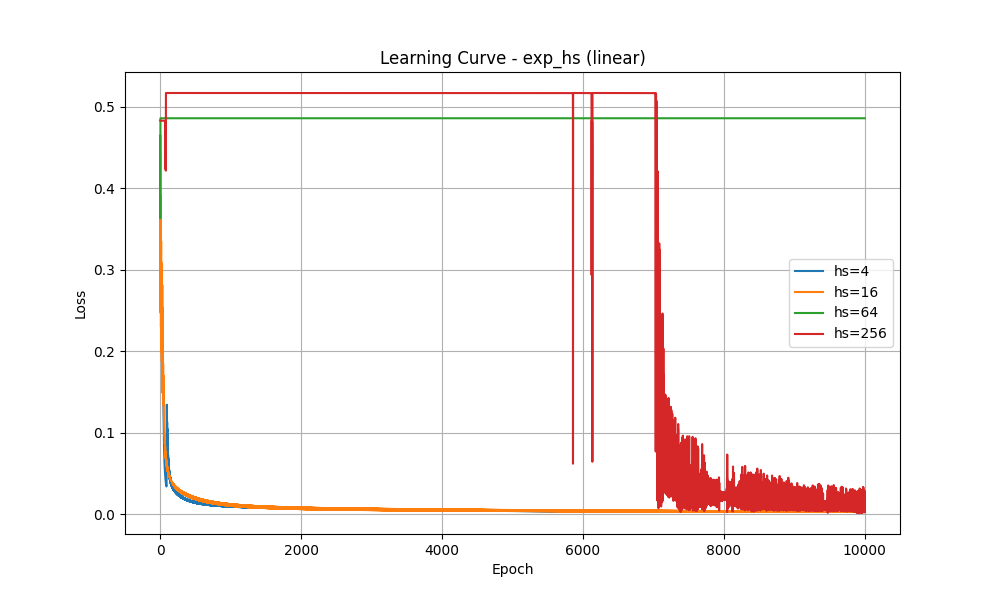
\includegraphics[width=\linewidth]{assets/learning_curve_exp_hs_linear.png}
  \caption{\textbf{Learning curves for different number of hidden units on linear dataset}}
  \label{fig:learning_curve_exp_hs_linear}
\end{figure}

\begin{figure}[H]
  \centering
  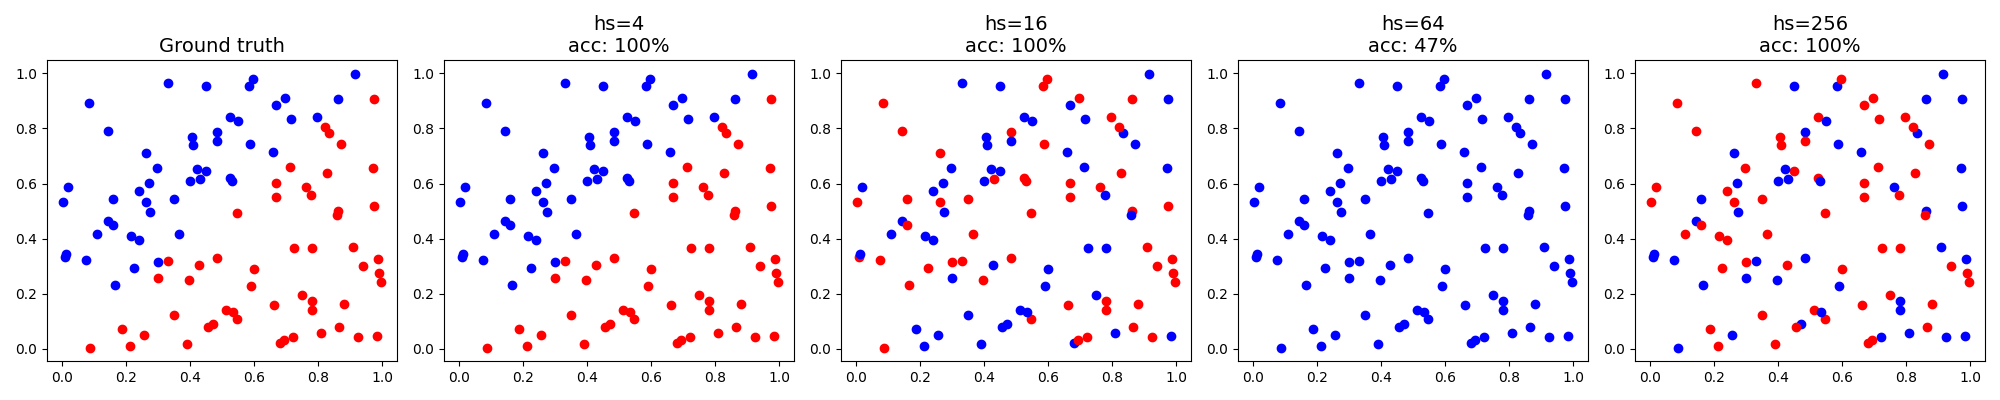
\includegraphics[width=\linewidth]{assets/result_exp_hs_linear.png}
  \caption{\textbf{Prediction results for different number of hidden units on linear dataset}}
  \label{fig:result_exp_hs_linear}
\end{figure}

% ----- Without Activation Functions -----

\subsection{Without Activation Functions}

Activation functions introduce the non-linearity required to solve the non-linear
question such as XOR. As shown in \cref{fig:learning_curve_exp_have_act_XOR} and 
\cref{fig:result_exp_have_act_XOR}, the model fails to converge on XOR dataset
without activation functions. In contrast, the model can still solve the linear
problem without activation functions (see \cref{fig:learning_curve_exp_have_act_linear} and 
\cref{fig:result_exp_have_act_linear}).

\begin{figure}[H]
  \centering
  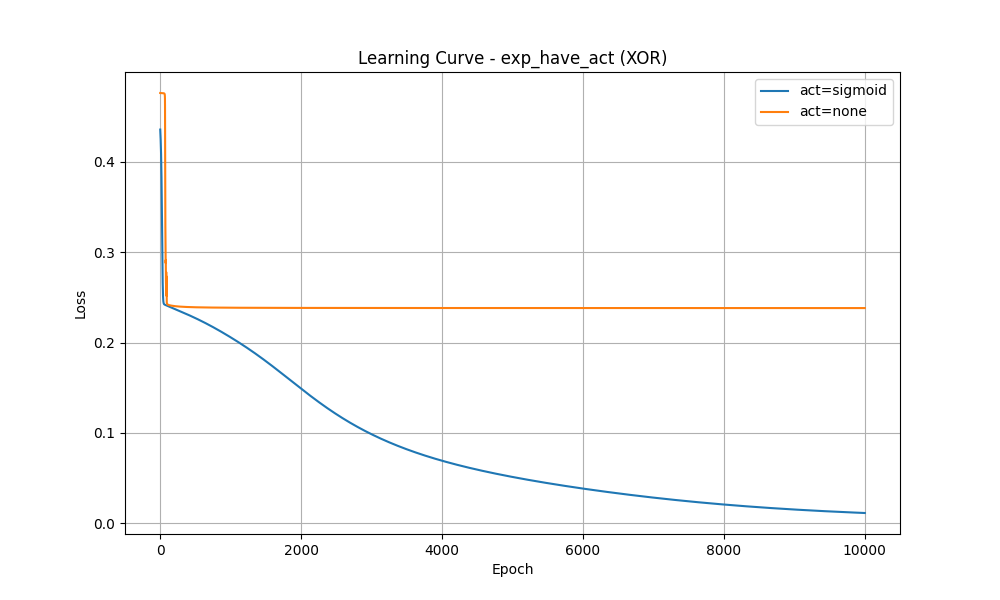
\includegraphics[width=\linewidth]{assets/learning_curve_exp_have_act_XOR.png}
  \caption{\textbf{Learning curves for XOR dataset with and without activation functions}}
  \label{fig:learning_curve_exp_have_act_XOR}
\end{figure}

\begin{figure}[H]
  \centering
  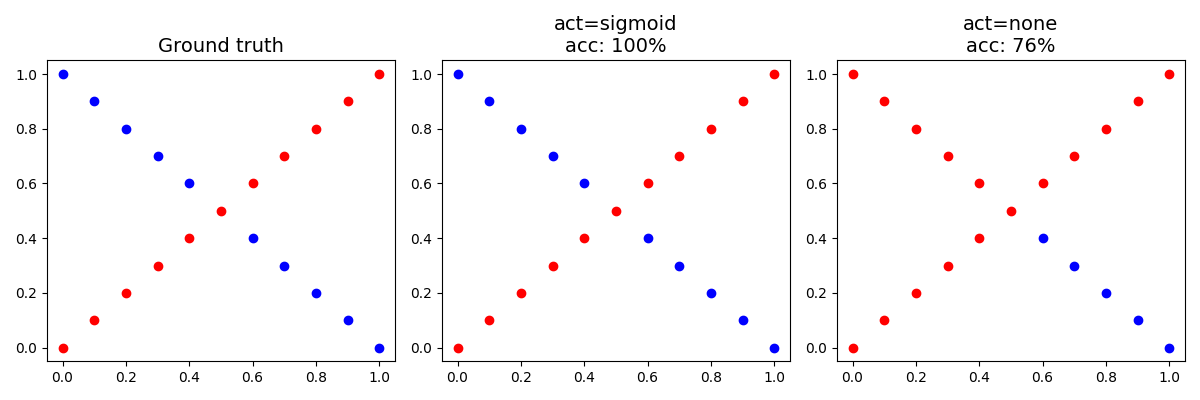
\includegraphics[width=\linewidth]{assets/result_exp_have_act_XOR.png}
  \caption{\textbf{Prediction results for XOR dataset with and without activation functions}}
  \label{fig:result_exp_have_act_XOR}
\end{figure}

\begin{figure}[H]
  \centering
  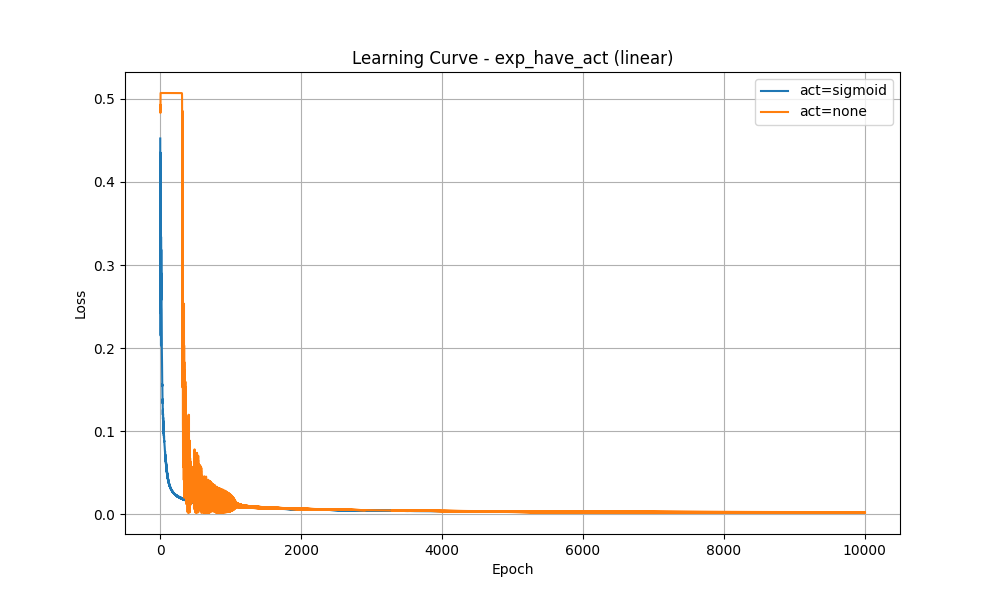
\includegraphics[width=\linewidth]{assets/learning_curve_exp_have_act_linear.png}
  \caption{\textbf{Learning curves for linear dataset with and without activation functions}}
  \label{fig:learning_curve_exp_have_act_linear}
\end{figure}

\begin{figure}[H]
  \centering
  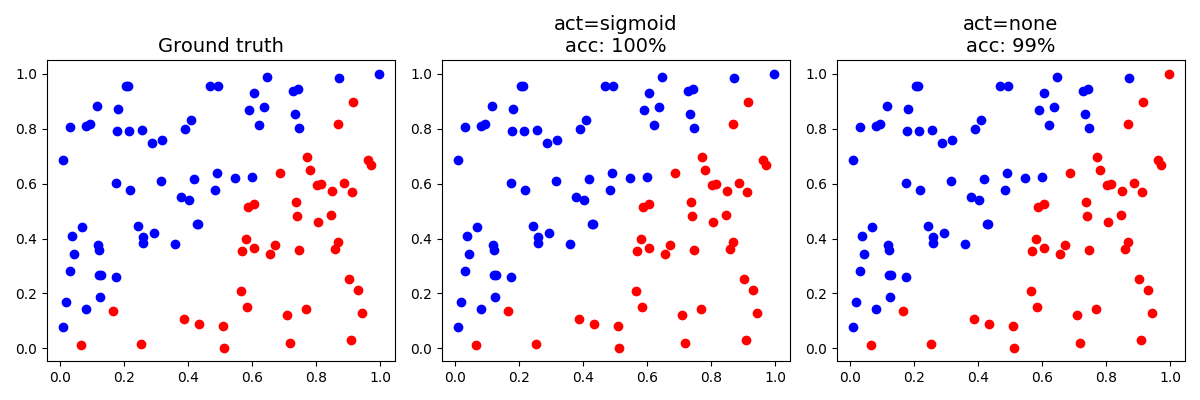
\includegraphics[width=\linewidth]{assets/result_exp_have_act_linear.png}
  \caption{\textbf{Prediction results for linear dataset with and without activation functions}}
  \label{fig:result_exp_have_act_linear}
\end{figure}

% --------------------------- Questions --------------------------

\section{Questions}

\subsection{Question 1}
\textbf{What is the purpose of activation functions?}

\textbf{Ans:} Activation functions introduce non-linearity into the
neural network. Without them, even a deep network with many layers
would just be a sequence of linear transformations, which is equivalent
to a single linear model. Non-linear activation functions (like
Sigmoid, ReLU, or Tanh) allow the model to learn and represent
complex boundaries, such as those required for the non-linearly
separable XOR dataset.

\subsection{Question 2}
\textbf{What might happen if the learning rate is too large or too small?}

\textbf{Ans:} If the learning rate is too large, the weight updates might
overshoot the global minimum, causing the loss to oscillate or even
diverge. It can also push weights into the saturation regions of
activation functions (vanishing gradients), as seen in the $\eta=0.1$
experiment. If the learning rate is too small, the convergence
becomes extremely slow, requiring an impractical number of epochs to
minimize the loss, and the model is more likely to get trapped in
poor local minima.

\subsection{Question 3}
\textbf{What is the purpose of weights and biases in a neural network?}

\textbf{Ans:} Weights ($W$) determine the relative importance or
influence of each input connection on the subsequent layer, essentially
scaling the signals to learn the underlying patterns. Biases ($b$) provide
an additive offset that allows the activation function to be shifted
horizontally. This shifting is crucial because it enables the network
to represent boundaries that do not necessarily pass through the
origin $(0,0)$, providing more flexibility in fitting the data.

% ----------------------------- Extra ----------------------------

\section{Extra}

\subsection{Different Activation Functions}

I compared \texttt{Sigmoid}, \texttt{ReLU}, and \texttt{Tanh}.
Note that these two tasks are both binary classification tasks, so
\texttt{Sigmoid} activation is used in the output layer no matter which
activation function is used internally. The results are shown in
\cref{fig:learning_curve_exp_act_XOR}, \cref{fig:result_exp_act_XOR},
\cref{fig:learning_curve_exp_act_linear}, and \cref{fig:result_exp_act_linear}.
\begin{itemize}
    \item \textbf{Sigmoid and Tanh:} Both functions squash the output into
      a bounded range ($(0,1)$ and $(-1,1)$ respectively). They successfully
      learn the XOR boundary and achieve $100\%$ accuracy. Tanh often converges
      faster than Sigmoid because its outputs are zero-centered, which aids
      gradient descent.
    \item \textbf{ReLU:} The model seems to be unstable and sensitive to the
      initial weights. Although it failed on linear dataset with the same setting
      as other experiments, I try different random seeds and find that it
      can converge with some values, as shown in \cref{tab:seed_relu}.
\end{itemize}

\begin{figure}[H]
  \centering
  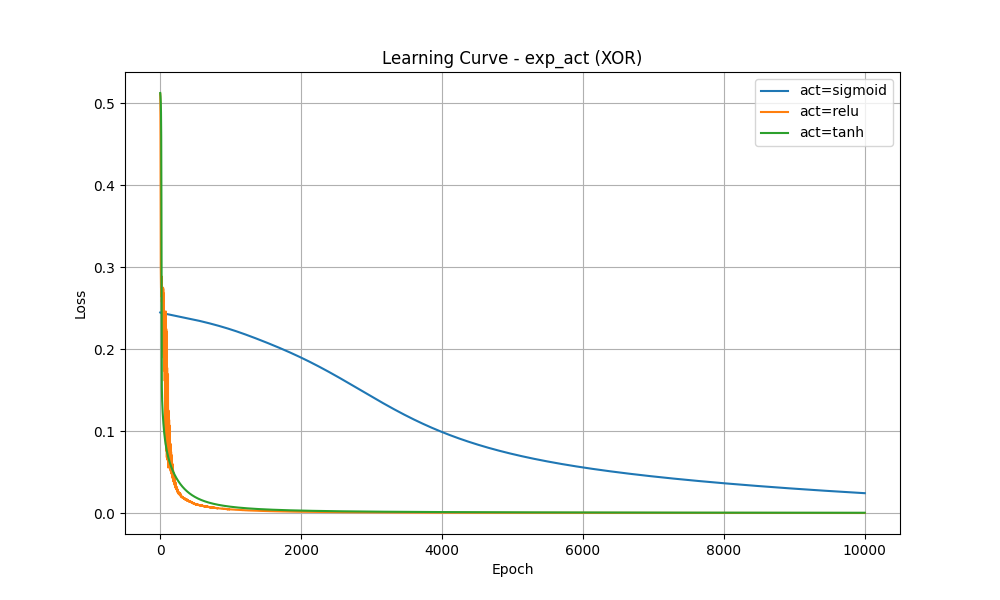
\includegraphics[width=\linewidth]{assets/learning_curve_exp_act_XOR.png}
  \caption{\textbf{Learning curves for different activation functions on XOR dataset}}
  \label{fig:learning_curve_exp_act_XOR}
\end{figure}

\begin{figure}[H]
  \centering
  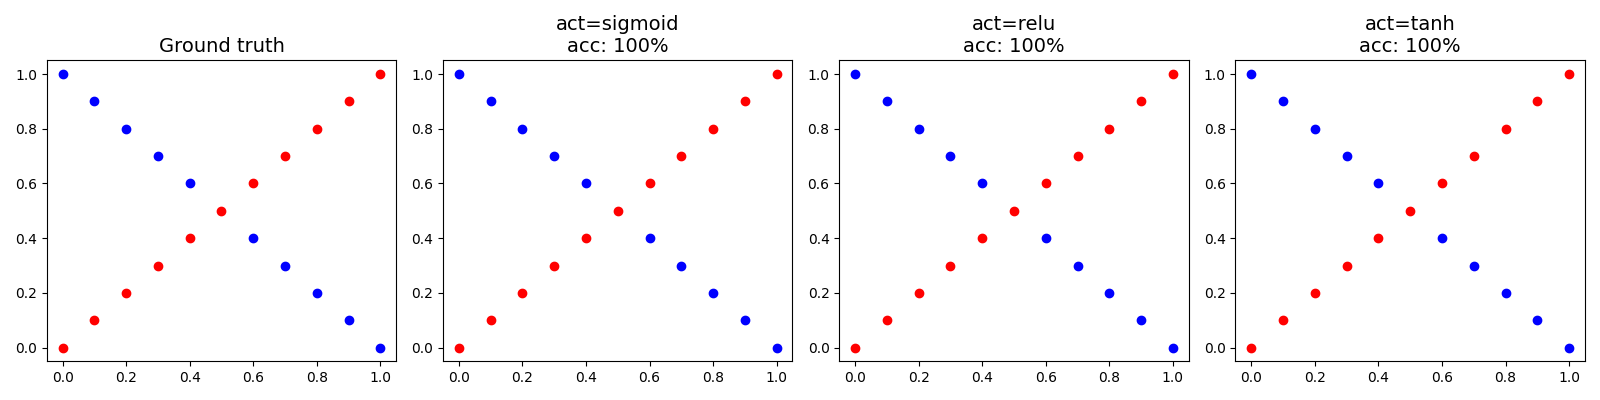
\includegraphics[width=\linewidth]{assets/result_exp_act_XOR.png}
  \caption{\textbf{Prediction results for different activation functions on XOR dataset}}
  \label{fig:result_exp_act_XOR}
\end{figure}

\begin{figure}[H]
  \centering
  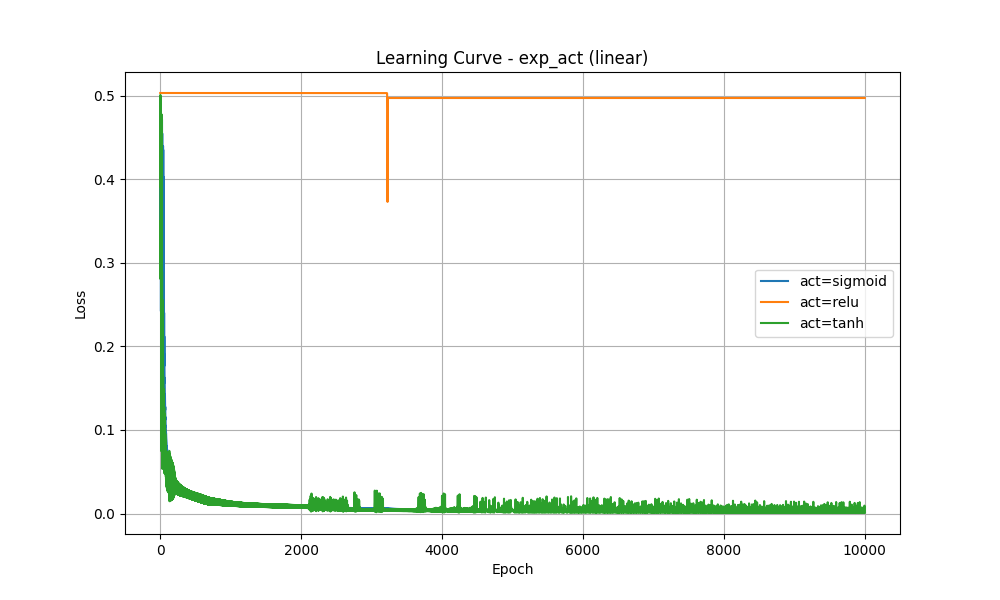
\includegraphics[width=\linewidth]{assets/learning_curve_exp_act_linear.png}
  \caption{\textbf{Learning curves for different activation functions on linear dataset}}
  \label{fig:learning_curve_exp_act_linear}
\end{figure}

\begin{figure}[H]
  \centering
  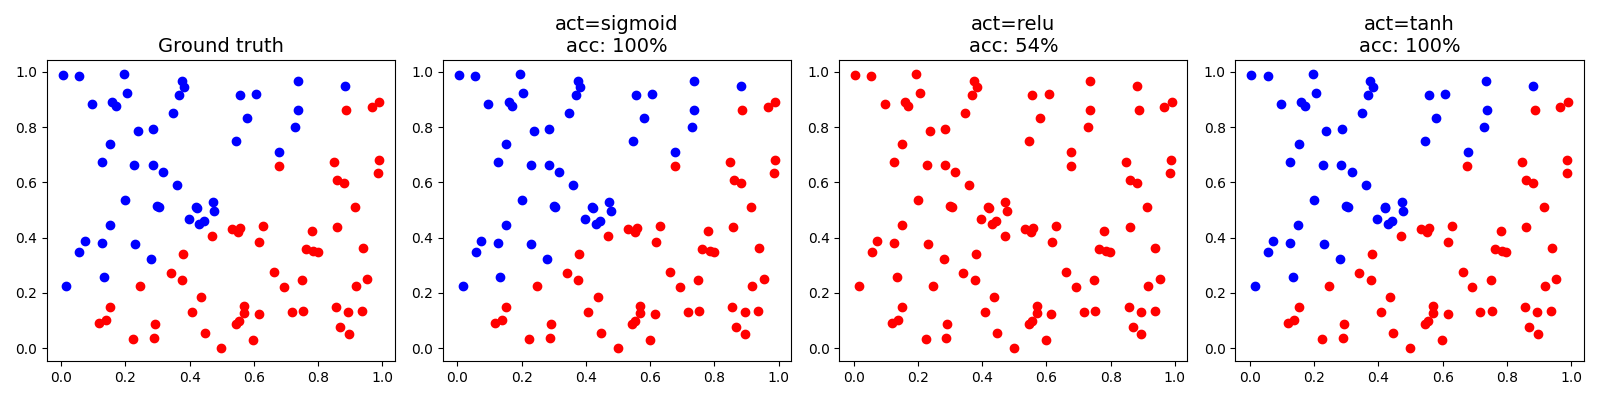
\includegraphics[width=\linewidth]{assets/result_exp_act_linear.png}
  \caption{\textbf{Prediction results for different activation functions on linear dataset}}
  \label{fig:result_exp_act_linear}
\end{figure}

\begin{table}[H]
  \centering
  \begin{tabular}{lccccc}
    \toprule
    seeds & 0 & 10 & 100 & 500 & 1000 \\
    \midrule
    acc. & $99\%$ & $46\%$ & $60\%$ & $99\%$ & $50\%$ \\
    \bottomrule
  \end{tabular}
  \caption{\textbf{Using different random seeds on linear dataset with ReLU activation function}}
  \label{tab:seed_relu}
\end{table}

% %%%%%%%%% REFERENCES %%%%%%%%%
% {\small
% \bibliographystyle{ieee_fullname}
% \bibliography{egbib}
% }

\end{document}